\section{Badania}
W~niniejszym rozdziale opisany został przebieg przeprowadzonych badań oraz analiza ich wyników. W~kolejnych podrozdziałach zostaną przedstawione różne przeprowadzone eksperymenty. Otrzymane wyniki znajdują się na~dołączonej do pracy płycie~CD w~odpowiednich plikach, o~nazwach zgodnych z~podrozdziałem opisującym dane badanie i~jego wyniki.

%\subsection{Opóźnienia pojedynczego odcinka sieci}
%\subsection{Wpływ topologi na opóźnienia}
\subsection{Czas stabilizacji sieci po odłączeniu i~podłączeniu dowolnego urządzenia}
Badanie miało na~celu sprawdzenie, czy zgodnie z~zapewnieniami producenta możliwe jest rozłączanie i~ponowne podłączanie urządzeń do~sieci ,,w locie'' bez konieczności dodatkowej ingerencji. Do przeprowadzenia pomiarów autor odłączał przewód ethernetowy i~podłączał go~ponownie do~gniazda. Oczywiście taka metoda może mieć wpływ na~dokładność dokonywanych pomiarów, ale zdaniem autora jest on stosunkowo niewielki, ze względu na fakt, że od~momentu odłączenia do wykrycia tego zajścia przez urządzenie nadzorujące pracę sieci, mija pewien czas, który w optymistycznym przypadku może być krótszy niż sam proces ingerencji autora. Aby poprawić dokładność należałoby zastosować samodzielnie stworzone urządzenie, co zostanie opisane w~perspektywach rozwoju niniejszej pracy. Wszystkie zmierzone czasy oraz treści komunikatów zostały odczytane w~środowisku TwinCAT System Manager, a przykładowy został przedstawiony na Rysunku~\ref{reading_time}.

\begin{figure}[!htb] 	\centering 	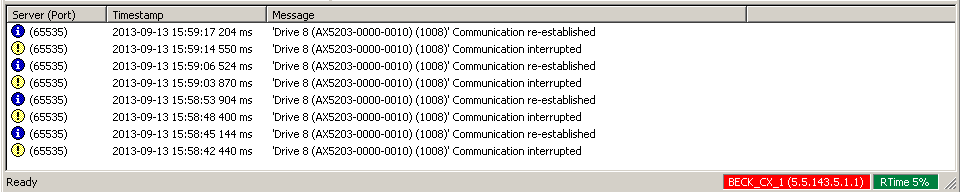
\includegraphics[width=0.99\textwidth]{images/reading_time} \caption{Topologia stanowiska z odłączonym jednym węzłem.} \label{reading_time} \end{figure}

\clearpage
\subsubsection{Pojedyncze urządzenie}
Eksperyment miał na~celu sprawdzenie, po upływie jakiego czasu od~odłączenia i~ponownego podłączenia pojedynczego węzła sieci zaczyna on~znów funkcjonować poprawnie. Zaburzoną pracę sieci przedstawiono na~Rysunku~\ref{one_slave}, który został wygenerowany przy użyciu środowiska TwinCAT System Manager, które udostępnia możliwość podglądu topologii sieci w~czasie rzeczywistym. Do eksperymentu wybrany został węzeł końcowy w~topologii.
\begin{figure}[!htb] 	\centering 	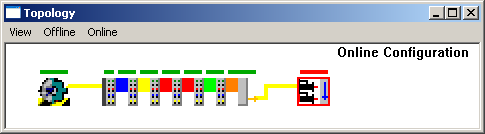
\includegraphics[width=0.9\textwidth]{images/topologyCXerror} \caption{Topologia stanowiska z odłączonym jednym węzłem.} \label{one_slave} \end{figure}

\begin{table}[!htb]
\begin{center}
\begin{tabular}{| c | c | c | c | c |}\hline
\textbf{Liczba} & \textbf{Wartość} & \textbf{Wartość} & \textbf{Wartość} & \textbf{Odchylenie} \\
\textbf{próbek} & \textbf{średnia} & \textbf{minimalna} & \textbf{maksymalna} & \textbf{standardowe} \\\hline\hline
20 & 2,715s & 2,644s & 3,184s & 0,131\\\hline
\end{tabular}
\end{center}
\vspace*{-6mm}
  \caption{Wyniki przeprowadzonego badania.}
	\label{badania:wyniki:stabilizacja_jeden}
\end{table}

\noindent Wyniki przeprowadzonego eksperymentu zostały zebrane w Tablicy~\ref{badania:wyniki:stabilizacja_jeden}. Na podstawie zmierzonych wartości oraz po ich analizie statystycznej uzyskano wykres przedstawiony na Rysunku~\ref{badania:wykres:stabilizacja_jeden}.

Analiza wyników przeprowadzonego badania potwierdza, że istnieje możliwość odłączenia i~ponownego podłączenia pojedynczego węzła sieci ,,w locie''. Czas potrzebny na~stabilizację połączenia po jego utracie jest zdaniem autora zadowalający. Obserwując uzyskany wykres można dojść do wniosku, że różnice pomiędzy kolejnymi iteracjami eksperymentu są stosunkowo małe, o czym świadczy odchylenie standardowe, którego wartość wynosi 0,131. Zdaniem autora głównym źródłem różnic jest zastosowana metoda pomiarowa.
\clearpage
\begin{figure}[htbp]
 \centering
 \begin{tikzpicture}[x=0.5cm,y=2cm]
  \tikzstyle{background grid}=[draw, black!50,step=.25cm]
	\draw[-latex, thin, draw=gray] (0,0)--(20,0) node [right] {$x$};
	\draw[-latex, thin, draw=gray] (0,0)--(0,4) node [above] {$t[s]$};
	%\draw [dotted, gray, step=0.5cm] (0,0) grid (20,4);
 
	\draw[thick] (0,2.678)--(20,2.678) node[left=10cm] {2,678};
	\draw[thin, dotted] (0,2.664)--(20,2.664) node[below] {min};
	\draw[thin, dotted] (0,2.774)--(20,2.774) node[above] {max};
		
	\node at (1, 2.664) {\textbullet};
	\node at (2, 2.664) {\textbullet};
	\node at (3, 2.654) {\textbullet};
	\node at (4, 2.664) {\textbullet};
	\node at (5, 2.654) {\textbullet};
	\node at (6, 2.774) {\textbullet};
	\node at (7, 2.764) {\textbullet};
	\node at (8, 2.664) {\textbullet};		
	\node at (9, 2.654) {\textbullet};
	\node at (10, 2.664) {\textbullet};
	\node at (11, 2.654) {\textbullet};
	\node at (12, 2.664) {\textbullet};
%	\node at (13, 2.774) {\textbullet};
%	\node at (14, 2.774) {\textbullet};
%	\node at (15, 2.774) {\textbullet};
%	\node at (16, 2.774) {\textbullet};							
%	\node at (17, 2.774) {\textbullet};
%	\node at (18, 2.774) {\textbullet};
%	\node at (19, 2.774) {\textbullet};
%	\node at (20, 2.774) {\textbullet};
					
\end{tikzpicture}
\caption{Pomiary czasu ponownego podłączenia oraz obliczona wartość średnia}
\label{badania:wykres:stabilizacja_jeden}
\end{figure}
\subsubsection{Wyspa z modułami I/O}
Eksperyment miał na~celu sprawdzenie po upływie jakiego czasu od~odłączeniu i~ponownego podłączenia zdalna wyspa z~dołączonymi kilkoma modułami wejścia/wyjścia zaczyna w~całości działać poprawnie tzn. wszystkie węzły nawiązują komunikację. Zaburzoną pracę sieci przedstawiono na~Rysunku~\ref{coupler}.
\begin{figure}[!htb] 	\centering 	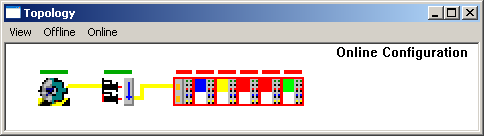
\includegraphics[width=0.8\textwidth]{images/topologyCPerror} \caption{Topologia stanowiska z odłączoną wyspą.} \label{coupler} \end{figure}
%1,5s wyspa i każdy kolejny moduł I/O z opóźnieniem 4ms

Wyniki przeprowadzonego eksperymentu zostały zebrane w Tablicy~\ref{badania:wyniki:stabilizacja_wyspa}.
\begin{table}[!htb]
\begin{center}
\begin{tabular}{| c | c | c | c | c |}\hline
\textbf{Liczba} & \textbf{Wartość} & \textbf{Wartość} & \textbf{Wartość} & \textbf{Odchylenie} \\
\textbf{próbek} & \textbf{średnia} & \textbf{minimalna} & \textbf{maksymalna} & \textbf{standardowe} \\\hline\hline
42 & 2,699s & 2,634s & 2,812s & 0,061s \\\hline
\end{tabular}
\end{center}
\vspace*{-6mm}
  \caption{Wyniki przeprowadzonego badania.}
	\label{badania:wyniki:stabilizacja_wyspa}
\end{table}

Na podstawie zmierzonych wartości oraz po ich analizie statystycznej uzyskano wykres przedstawiony na Rysunku~\ref{badania:wykres:stabilizacja_wyspa}. Różnymi kolorami są oznaczone kolejne iteracje badania, a~punkty tego samego koloru oznaczają kolejne węzły zdalnej stacji wejść/wyjść.
\begin{figure}[htbp]
 \centering
 \begin{tikzpicture}[x=0.5cm,y=10cm]


 \draw[latex-latex, thin, draw=gray] (0,1.25)--(20,1.25) node [right] {$x$}; % l'axe des abscisses
 \draw[latex-latex, thin, draw=gray] (0,1.25)--(0,2) node [above] {$y$}; % l'axe des ordonnées
 \draw[thick] (0,1.5)--(20,1.58); % l'axe des abscisses

    \foreach \i in {0,...,20}{% 
\foreach \Point in {(\i ,1.5+0.004*\i)}{
    \node at \Point {\textbullet}; } ;}     

% to ensure that the points are being properly centered:
\draw [dotted, gray] (0,1.25) grid (20,2);

\end{tikzpicture}
\caption{Współczynnik wykorzystania kanału transmisyjnego w Ethernecie (dwa pierwsze wykresy od lewej strony) i EtherCAT}
\label{etherCAT:wykorzystanie}
\end{figure}

Spoglądając na uzyskane wyniki oraz wykres można zaobserwować, że zwiększenie liczby odłączanych i~podłączanych ponownie węzłów nie~wpłynęło na~możliwość dokonywania tej operacji w~czasie pracy sieci. Ciekawa zdaniem autora jest różnica czasu pomiędzy podłączeniem się pierwszego urządzenia z~zestawu, a~każdym kolejnym wynoszący 2 lub 4 milisekundy. Tak więc, liczba modułów wejścia/wyjścia ma~proporcjonalnie niewielki wpływ na czas potrzebny do ustabilizowania się całego zdalnego zestawu.

\subsubsection{Wszystkie węzły sieci}
\label{badania:cala_siec}
Eksperyment miał na~celu sprawdzenie, po upływie jakiego czasu od~odłączeniu i~ponownego podłączenia wszystkich węzłów sieci, wróci ona do~normalnego stanu. Zaburzoną pracę sieci przedstawiono na~Rysunku~\ref{topologyCPallerror}.
\begin{figure}[!htb] 	\centering 	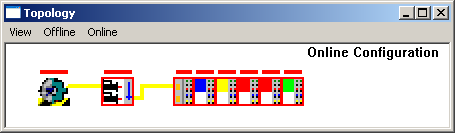
\includegraphics[width=0.9\textwidth]{images/topologyCPallerror} \caption{Topologia stanowiska z odłączonymi wszystkimi węzłami.} \label{topologyCPallerror} \end{figure}

\noindent Stan sieci bezpośrednio po ponownym podłączeniu kabla sieciowego i~w~fazie inicjalizacji ponownego połączenia przedstawiono na Rysunku~\ref{topologyCPallloading}. Można zaobserwować, że węzły połączone w~zdalną stację wejść/wyjść są już w~jednej z~kolejnych faz inicjalizacji, a~pozostałe jeszcze jej nie rozpoczęły.
\begin{figure}[!htb] 	\centering 	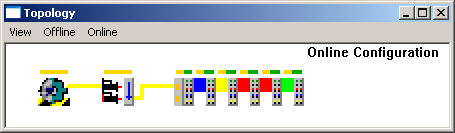
\includegraphics[width=0.9\textwidth]{images/topologyCPallloading} \caption{Topologia stanowiska w czasie ponownego podłączania węzłów.} \label{topologyCPallloading} \end{figure}

\begin{table}[!htb]
\begin{center}
\begin{tabular}{| c | c | c | c | c |}\hline
\textbf{Liczba} & \textbf{Wartość} & \textbf{Wartość} & \textbf{Wartość} & \textbf{Odchylenie} \\
\textbf{próbek} & \textbf{średnia} & \textbf{minimalna} & \textbf{maksymalna} & \textbf{standardowe} \\\hline\hline
10 & 4,790s & 4,149s & 5,455s & 0,446s\\\hline
\end{tabular}
\end{center}
\vspace*{-6mm}
  \caption{Wyniki przeprowadzonego badania.}
	\label{badania:wyniki:stabilizacja_siec}
\end{table}

\noindent Wyniki przeprowadzonego eksperymentu zostały zebrane w Tablicy~\ref{badania:wyniki:stabilizacja_jeden}. Na podstawie zmierzonych wartości oraz po ich analizie statystycznej uzyskano wykres przedstawiony na Rysunku~\ref{badania:wykres:stabilizacja_siec}.
\begin{figure}[h]
 \centering
 \begin{tikzpicture}[x=1cm,y=5cm]
  \tikzstyle{background grid}=[draw, black!50,step=.25cm]
	\draw[-latex, thin, draw=gray] (0,4)--(10,4) node [right] {$x$};
	\draw[-latex, thin, draw=gray] (0,3.95)--(0,5.55) node [left] {$t[s]$};
	%\draw [dotted, gray, step=0.5cm] (0,0) grid (20,4);
 	\draw (0,4) node[left] {4};
	\draw[] (0,4.790)--(10,4.790) node[left=10cm] {4,790};
	\draw[thin, dotted] (0,4.149)--(10,4.149) node[below] {min};
	\draw[thin, dotted] (0,5.455)--(10,5.455) node[above] {max};
		
	\node at (1, 4.863) {\textbullet};
	\node at (2, 4.149) {\textbullet};
	\node at (3, 5.313) {\textbullet};
	\node at (4, 5.455) {\textbullet};
	\node at (5, 4.339) {\textbullet};
	\node at (6, 4.911) {\textbullet};
	\node at (7, 5.099) {\textbullet};
	\node at (8, 4.339) {\textbullet};		
	\node at (9, 4.967) {\textbullet};
	\node at (10, 4.463) {\textbullet};
					
\end{tikzpicture}
\caption{Pomiary czasu ponownego podłączenia oraz obliczona wartość średnia.}
\label{badania:wykres:stabilizacja_siec}
\end{figure}

Analiza wyników przeprowadzonego badania pozwala wysnuć wniosek, że możliwe jest całkowite rozłączenie i~ponowne podłączenie sieci ,,w locie''. Czas potrzebny na~stabilizację połączenia po jego utracie również w tym wypadku jest zdaniem autora zadowalający. Niestety jednak porównując uzyskane wielkości do~tych z~badania pojedynczego węzła sieci można zauważyć, że czas ten wzrósł dość znacząco i~w~przypadku jeszcze większej liczby węzłów przestanie on już być akceptowalny. Obserwując uzyskany wykres można dojść do wniosku, że różnice pomiędzy kolejnymi iteracjami eksperymentu są stosunkowo małe i~wpływ na~nie może mieć w~większości zastosowana metoda pomiarowa.

\subsubsection{Pełna stabilizacja urządzenia}
W~czasie badań autor zauważył, że zmierzone w~pierwszych trzech eksperymentach czasy określają jedynie czas potrzebny na ustabilizowanie sieci, ale nie uwzględniają tego, że po nawiązaniu połączenia urządzenie wymaga jeszcze pewnego czasu na ustawienie się w~prawidłowy stan 'Operational'. Eksperyment ten został przeprowadzony z~wykorzystaniem stworzonego oprogramowania oraz wizualizacji. Autor dokonał pomiaru czasu od momentu zmiany stanu urządzenia z~OP, aż do jego powrotu do prawidłowego stanu.

\begin{table}[!htb]
\begin{center}
\begin{tabular}{| c | c | c | c | c |}\hline
\textbf{Liczba} & \textbf{Wartość} & \textbf{Wartość} & \textbf{Wartość} & \textbf{Odchylenie} \\
\textbf{próbek} & \textbf{średnia} & \textbf{minimalna} & \textbf{maksymalna} & \textbf{standardowe} \\\hline\hline
20 & 5,646s & 5,440s & 6,080s & 0,165\\\hline
\end{tabular}
\end{center}
\vspace*{-6mm}
  \caption{Wyniki przeprowadzonego badania.}
	\label{badania:wyniki:op_jeden}
\end{table}

\noindent Wyniki przeprowadzonego eksperymentu zostały zebrane w Tablicy~\ref{badania:wyniki:op_jeden}. Na podstawie zmierzonych wartości oraz po ich analizie statystycznej uzyskano wykres przedstawiony na Rysunku~\ref{badania:wykres:op_jeden}.
\begin{figure}[h]
 \centering
 \begin{tikzpicture}[x=0.5cm,y=10cm]
  \tikzstyle{background grid}=[draw, black!50,step=.25cm]
	\draw[-latex, thin, draw=gray] (0,5.3)--(20,5.3) node [right] {$x$};
	\draw[-latex, thin, draw=gray] (0,5.25)--(0,6.15) node [left] {$t[s]$};
	%\draw [dotted, gray, step=0.5cm] (0,0) grid (20,4);
 	\draw (0,5.3) node[left] {5,3};
	\draw[] (0,5.646)--(20,5.646) node[left=10cm] {5,646};
	\draw[thin, dotted] (0,5.440)--(20,5.440) node[below] {min};
	\draw[thin, dotted] (0,6.080)--(20,6.080) node[above] {max};
		
	\node at (1, 5.480) {\textbullet};
	\node at (2, 5.770) {\textbullet};
	\node at (3, 5.660) {\textbullet};
	\node at (4, 5.630) {\textbullet};
	\node at (5, 5.630) {\textbullet};
	\node at (6, 5.530) {\textbullet};
	\node at (7, 5.440) {\textbullet};
	\node at (8, 6.080) {\textbullet};		
	\node at (9, 5.550) {\textbullet};
	\node at (10, 5.560) {\textbullet};
	\node at (11, 5.760) {\textbullet};
	\node at (12, 5.730) {\textbullet};
	\node at (13, 5.460) {\textbullet};
	\node at (14, 5.720) {\textbullet};
	\node at (15, 5.530) {\textbullet};
	\node at (16, 5.870) {\textbullet};							
	\node at (17, 5.790) {\textbullet};
	\node at (18, 5.510) {\textbullet};
	\node at (19, 5.760) {\textbullet};
	\node at (20, 5.450) {\textbullet};
					
\end{tikzpicture}
\caption{Pomiary czasu ponownego podłączenia oraz obliczona wartość średnia.}
\label{badania:wykres:op_jeden}
\end{figure}

Analiza wyników przeprowadzonego badania wykazuje, że czas potrzebny na przywrócenie węzła do prawidłowego działania jest dwukrotnie wyższy niż w~przypadku odzyskiwania połączenia. Czas potrzebny na stabilizację połączenia po jego utracie jest zdaniem autora zadowalający, ale już nie tak dobry jak czas stabilizacji połączenia. Obserwując uzyskany wykres można dojść do wniosku, że różnice pomiędzy kolejnymi iteracjami eksperymentu są stosunkowo małe, o czym świadczy odchylenie standardowe, którego wartość wynosi 0,165. Zdaniem autora głównym źródłem różnic jest zastosowana metoda pomiarowa.

Dodatkowym wynikiem badania jest wykrycie faktu, że oprócz odłączonego węzła stan swój zmienia węzeł będący terminalem przyłączeniowym (EK1100). Fakt ten nie zostaje wykryty i~zgłoszony przez środowisko oraz nie był widoczny na podglądzie topologii w~czasie zaburzania. Autor postanowił przebadać i~przeanalizować czas potrzebny na powrót tego węzła do prawidłowego działania. Fakt ten może mieć duże znaczenie przy innych topologiach, gdzie do jednego terminala będzie podłączonych więcej węzłów podrzędnych. W~takiej sytuacji autor przewiduje przerwanie komunikacji z~wszystkimi węzłami podpiętymi do terminala.

\begin{table}[!htb]
\begin{center}
\begin{tabular}{| c | c | c | c | c |}\hline
\textbf{Liczba} & \textbf{Wartość} & \textbf{Wartość} & \textbf{Wartość} & \textbf{Odchylenie} \\
\textbf{próbek} & \textbf{średnia} & \textbf{minimalna} & \textbf{maksymalna} & \textbf{standardowe} \\\hline\hline
10 & 1,653s & 1,570s & 1,870s & 0,091\\\hline
\end{tabular}
\end{center}
\vspace*{-6mm}
  \caption{Wyniki przeprowadzonego badania.}
	\label{badania:wyniki:op_jeden_bonus}
\end{table}

\noindent Wyniki przeprowadzonego eksperymentu zostały zebrane w Tablicy~\ref{badania:wyniki:op_jeden_bonus}. Na podstawie zmierzonych wartości oraz po ich analizie statystycznej uzyskano wykres przedstawiony na Rysunku~\ref{badania:wykres:op_jeden_bonus}.
\begin{figure}[h]
 \centering
 \begin{tikzpicture}[x=1cm,y=10cm]
  \tikzstyle{background grid}=[draw, black!50,step=.25cm]
	\draw[-latex, thin, draw=gray] (0,1.5)--(10,1.5) node [right] {$x$};
	\draw[-latex, thin, draw=gray] (0,1.45)--(0,2) node [left] {$t[s]$};
	%\draw [dotted, gray, step=0.5cm] (0,0) grid (20,4);
 	\draw (0,1.5) node[left] {1,5};
	\draw[] (0,1.653)--(10,1.653) node[left=10cm] {1,653};
	\draw[thin, dotted] (0,1.570)--(10,1.570) node[below] {min};
	\draw[thin, dotted] (0,1.870)--(10,1.870) node[above] {max};
		
	\node at (1, 1.590) {\textbullet};
	\node at (2, 1.870) {\textbullet};
	\node at (3, 1.610) {\textbullet};
	\node at (4, 1.650) {\textbullet};
	\node at (5, 1.750) {\textbullet};
	\node at (6, 1.600) {\textbullet};
	\node at (7, 1.610) {\textbullet};
	\node at (8, 1.640) {\textbullet};		
	\node at (9, 1.570) {\textbullet};
	\node at (10, 1.640) {\textbullet};
					
\end{tikzpicture}
\caption{Pomiary czasu ponownego podłączenia oraz obliczona wartość średnia.}
\label{badania:wykres:op_jeden_bonus}
\end{figure}

Wyniki przeprowadzonego eksperymentu mają taką samą charakterystykę jak we wszystkich dotychczasowych badaniach. Czas powrotu do prawidłowego stanu pracy w~tym przypadku jest aż trzy razy mniejszy niż dla węzła odłączanego. Zdaniem autora wynika to z~prostszego oprogramowania wewnętrznego terminala przyłączeniowego (emulowana maszyna stanów) lub węzeł zaburzony rozpoczyna swoją potencjalizację po węźle poprzedzającym.

\subsubsection{Problemy}
W~czasie dziesiątek przeprowadzonych w~tym badaniu pomiarów autor doprowadził do sytuacji, w~której sieć nie~powróciła już samoczynnie do~prawidłowego działania. Jest to sprzeczne z~zapewnieniami twórców standardu i~dlatego przypadek ten zostanie tu szczegółowo opisany i~przeanalizowany.

%\begin{enumerate}
%\item 
Treść wiadomości odczytanej ze środowiska była następująca: \textit{Device 2 (EtherCAT (v2.10 only)': 'INIT to PREOP' failed! Error: 'read slave count'. Communication Error '0x707 (1799)'.}
Do błędu doszło w~momencie zaburzenia pracy całej sieci, tj. odłączenia wszystkich węzłów podrzędnych od węzła nadrzędnego jak w~badaniu~\ref{badania:cala_siec}. Stan sieci po~wystąpieniu błędu przedstawiono na Rysunku~\ref{err0x707}.
\begin{figure}[!htb] 	\centering 	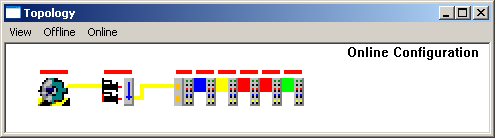
\includegraphics[width=0.9\textwidth]{images/err0x707} \caption{Stan sieci po błędzie 0x707.} \label{err0x707} \end{figure}

Na rysunku można zaobserwować, że urządzenia są podłączone do sieci, ale ich stan jest błędny (brak czerwony ramek wokół węzłów). Analizując stan stanowiska i~sieci w~środowisku zaobserwowano, że w~sieci nie są przesyłane dane.
Dalsza analiza wykazała, że węzeł AX-5203 jest w prawidłowym stanie inicjalizacji (0x0001), natomiast problematyczna okazała się zdalna wyspa, która ma nieprawidłowy stan 0x5C01, który według jednej z dokumentacji producenta oznacza błąd podczas resetowania stanu \cite{err0x707}.
Okazało się, ze problem ten można prosto rozwiązać bez potrzeby restartowania całego stanowiska poprzez wymuszenie zmiany stanu węzła nadrzędnego z~INIT na~OP (opcja dostępna z~poziomu środowiska), co skutkuje wysłaniem takiego samego żądania do wszystkich węzłów podrzędnych i sieć ponownie zaczyna funkcjonować. Wynik analizy znajduje odzwierciedlenie bezpośrednio w~treści wiadomości opisującej błąd.
%\end{enumerate}

Podsumowując wszystkie powyższe badania przeprowadzone w~tym podrozdziale autor wyciągnął dwa kluczowe wnioski:
\begin{enumerate}
\item odłączanie oraz ponowne podłączanie pojedynczego węzła, grupy węzłów, a~nawet całej sieci jest możliwe ,,w~locie'' w~pracującym systemie; należy jednak pamiętać, że operacja stabilizacji sieci oraz przywracanie urządzeń do prawidłowego stanu wymaga czasu i~w~przypadku nie wszystkich instalacji będzie to dopuszczalne,
\item należy pamiętać, że jeżeli w~czasie przywracania prawidłowego stanu sieci jakiekolwiek urządzenie nie przejdzie prawidłowo ze stanu inicjalizacji do stanu operacyjnego to~działanie całej sieci zostaje zawieszone.
\end{enumerate}
\subsection{Opóźnienie transmisji}
Eksperyment miał na celu sprawdzenie, czy w~protokole występują opóźnienia związane z~transmisją danych. Dla przebadania autor postanowił zastosować dostępne na stanowisku serwomechanizmy. Jako fundament wykorzystano podstawową konfigurację sterowników i wizualizację. Do badania wykorzystano po~jednym serwomechanizmie z~każdego stanowiska, a~do ich sterowania zastosowano dostępny z~poziomu TwinCAT System Managera moduł TwinCAT NC Server, którego przykładowy wygląda przedstawiono na Rysunku~\ref{axis_function}. Zastosowanie tej metody było uzasadnione tym, że obserwując zmienne związane z~pracą silnika autor dostrzegł, że odpowiednie parametry są regularnie przetwarzane i wymieniane pomiędzy jednostką centralną, a napędem. Duża ilość przesyłanych danych sugeruje, że jeżeli występują jakieś opóźnienia w~transmisji to eksperyment powinien je wykazać.

\begin{figure}[!htb] 	\centering 	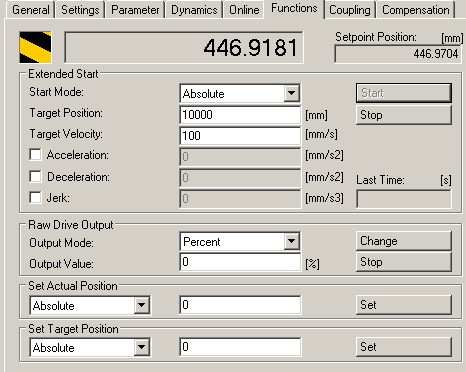
\includegraphics[width=0.85\textwidth]{images/axis_function} \caption{Moduł pozwalający sterować silnikiem z~wykorzystaniem funkcji.} \label{axis_function} \end{figure}

Autor zadawał różne funkcje podając pozycje docelowe oraz żądaną prędkość. Wykorzystując stworzone oprogramowanie oraz wizualizację mierzono czas trwania ruchu silnika. Te same zadania były równolegle uruchamiane na obu stanowiskach. Autor zawsze przeprowadzał pomiar dwukrotnie tzn. od pozycji zerowej do pozycji docelowej i~z~powrotem żeby wykluczyć przypadkowe różnice. Wiele kombinacji odległości i~prędkości poskutkowało uzyskiwaniem czasów od pojedynczych sekund do kilku minut. 

\noindent Niestety badanie to nie wykazało żadnych opóźnień w~transmisji, ponieważ:
\begin{itemize}
\item czasy tam i~z~powrotem w każdej próbie były równe,
\item czasy odmierzane na dwóch niezależnych stanowiskach o~różnej topologii oraz liczbie węzłów podrzędnych zawsze były równe.
\end{itemize}

Autor dokładał wszelkich starań, aby uzyskać rozbieżne wyniki, ale dalsze wydłużanie czasu pracy silników nie przynosiło efektów. Nawet odłączanie i~ponowne podłączanie zdalnych modułów wejścia/wyjścia w~czasie pracy silnika nie wpłynęło na otrzymywane wyniki. Dodatkowo autor przeprowadził to samo badanie wykorzystując stanowisko rozszerzone do 15 węzłów slave, ale również w~tym przypadku osiągane wyniki nie wykazały występowania opóźnień transmisji.
%\subsubsection{Zbadanie innych topologii}
%\subsubsection{Zbadanie opóźnień na poziomie transmisji pojedynczych ramek}
%Różne kable
%Długość kabla
%
%Połączyć do jednego sterownika oba napędy kolejno i zrobić coś na zasadzie inkrementacji i sprawdzić czy się przypadkiem nie rozjedzie
%
%Mamy opóźnienie na jednym odcinku
%
%Ewentualnie jeden kabel można zamienić na dłuższy i sprawdzić czy nie ma różnicy.
%
%Wymyślić jak sprawdzić czas ponownego włączenia do sieci.